\chapter{مقدمه}
\section{پیش‌گفتار}
این نمونه‌ای از زیرنویس \LTRfootnote{English Footnote} انگلیسی است.	
این نمونه‌ای از زیرنویس \LTRfootnote{English Footnote} انگلیسی است.	
در این قالب سعی شده است که از تمامی بخش‌های موجود در پایان‌نامه‌ها نمونه‌ای آورده شود. در این قالب سعی شده است که از تمامی بخش‌های موجود در پایان‌نامه‌ها نمونه‌ای آورده شود. در این قالب سعی شده است که از تمامی بخش‌های موجود در پایان‌نامه‌ها نمونه‌ای آورده شود. در این قالب سعی شده است که از تمامی بخش‌های موجود در پایان‌نامه‌ها نمونه‌ای آورده شود. در این قالب سعی شده است که از تمامی بخش‌های موجود در پایان‌نامه‌ها نمونه‌ای آورده شود. در این قالب سعی شده است که از تمامی بخش‌های موجود در پایان‌نامه‌ها نمونه‌ای آورده شود. در این قالب سعی شده است که از تمامی بخش‌های موجود در پایان‌نامه‌ها نمونه‌ای آورده شود. در این قالب سعی شده است که از تمامی بخش‌های موجود در پایان‌نامه‌ها نمونه‌ای آورده شود. در این قالب سعی شده است که از تمامی بخش‌های موجود در پایان‌نامه‌ها نمونه‌ای آورده شود. در این قالب سعی شده است که از تمامی بخش‌های موجود در پایان‌نامه‌ها نمونه‌ای آورده شود. در این قالب سعی شده است که از تمامی بخش‌های موجود در پایان‌نامه‌ها نمونه‌ای آورده شود. در این قالب سعی شده است که از تمامی بخش‌های موجود در پایان‌نامه‌ها نمونه‌ای آورده شود. در این قالب سعی شده است که از تمامی بخش‌های موجود در پایان‌نامه‌ها نمونه‌ای آورده شود. در این قالب سعی شده است که از تمامی بخش‌های موجود در پایان‌نامه‌ها نمونه‌ای آورده شود.
\section{بخش اول}
نمونه‌ای از یک عبارت انگلیسی در متن به‌صورت

\lr{English Sentence}
است. نمونه‌ای از یک عبارت ریاضی در متن نیز به‌صورت
$x^2 + y^2$
است. ارجاع به مراجع انگلیسی
\cite{Fakhari2015a,Lewis2003}.
ارجاع به مراجع فارسی
\cite{Fakhari2015b,HadianThesis2008}.
این نمونه‌ای از یک زیرنویس انگلیسی%
\LTRfootnote{English Footnote}
است. این نمونه‌ای از یک زیرنویس فارسی%
\RTLfootnote{زیرنویس فارسی}
است. در شکل
\ref{Fig:SampleFigure1}،
نمونه‌ای از یک شکل آورده شده است. 

\begin{figure}[!htb]
\centering
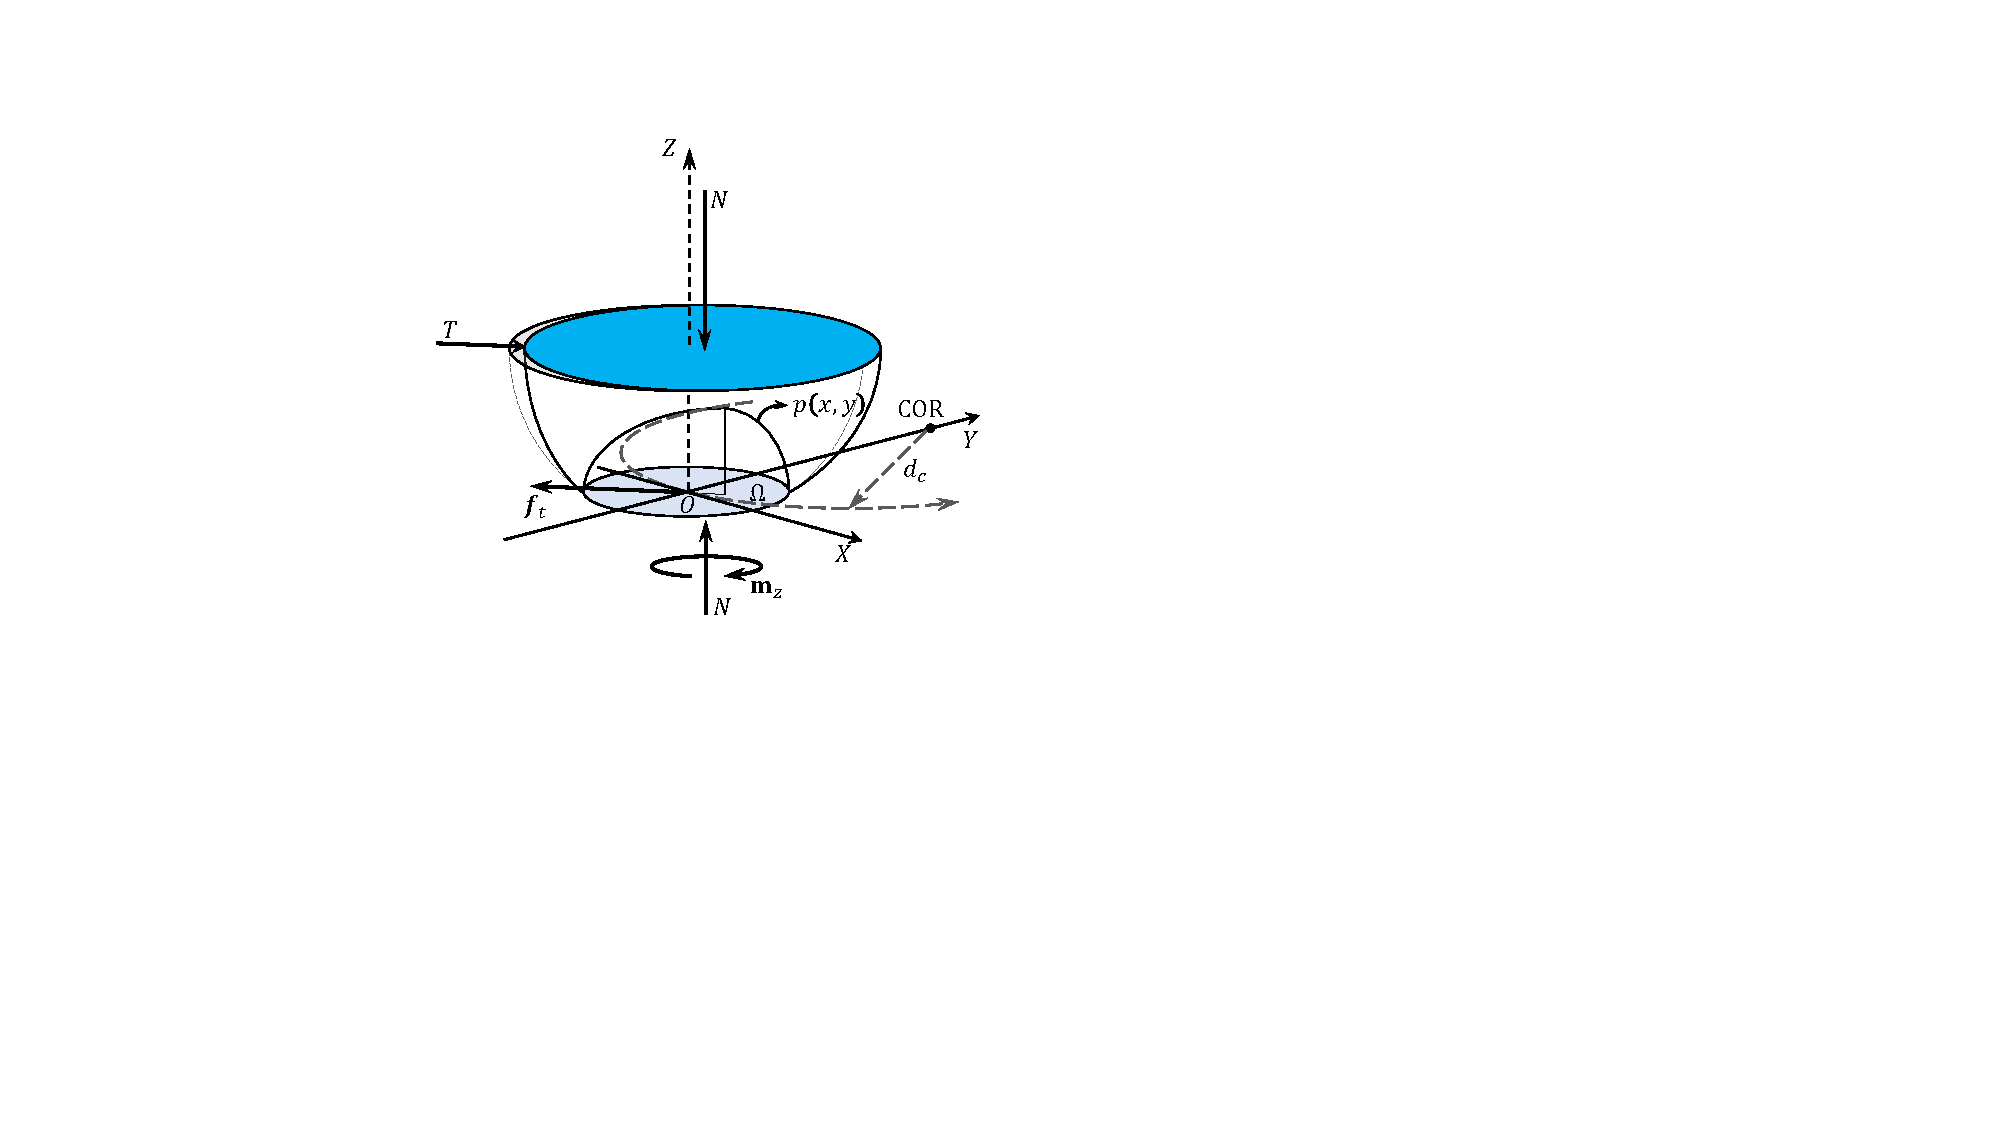
\includegraphics[scale=1]{Figures/SampleFigure.pdf}
\caption{شکل نمونه}
\label{Fig:SampleFigure1}
\end{figure}

نمونه‌ای از قرار دادن دو شکل در کنار یکدیگر در شکل
\ref{Fig:SampleFigure2}
آورده شده است.

\begin{figure}[!htb]
\centering
\subfloat[زیرنویس شکل اول]{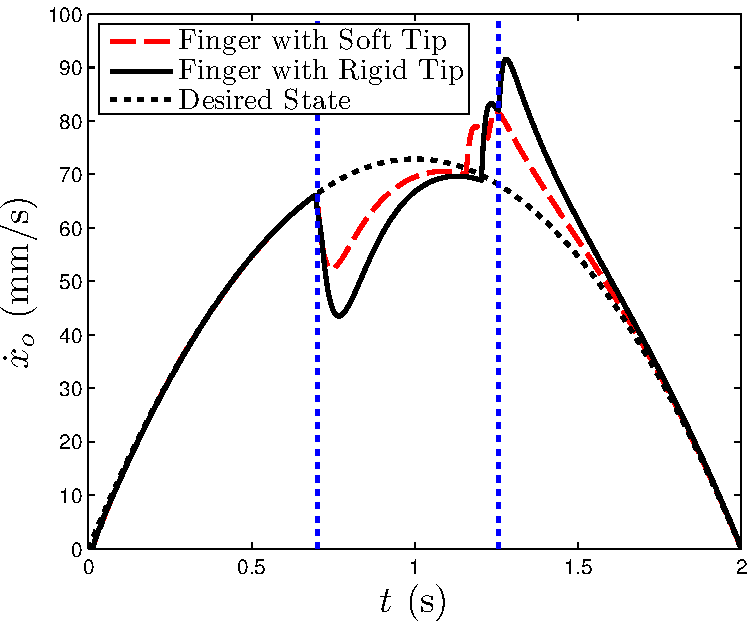
\includegraphics[scale=0.56]{Figures/FigureA.pdf}}
\quad
\subfloat[زیرنویس شکل دوم]{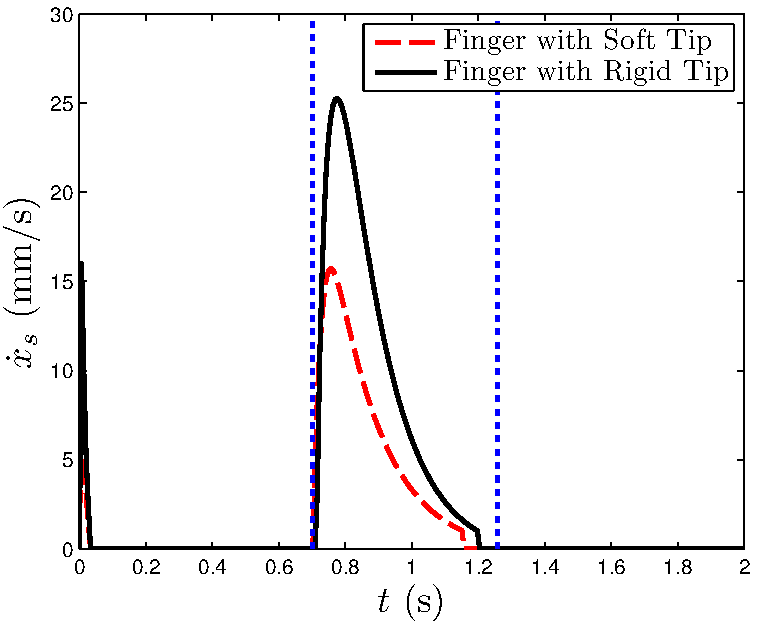
\includegraphics[scale=0.56]{Figures/FigureB.pdf}}
\caption{
قرار دادن دو شکل در کنار یکدیگر، الف) شکل نمونه اول،
ب) شکل نمونه دوم
}
\label{Fig:SampleFigure2}
\end{figure}





آیتم‌های مختلف به‌صورت زیر آورده می‌شود:
\begin{itemize}[label=-]
\item
مورد اول
\item
مورد دوم
\item
مورد سوم
\end{itemize}

نمونه‌ای از آیتم‌های شماره‌دار نیز در ادامه آورده شده است. به طور کلی معماری برداشت انرژی به دو دسته‌ی کلی تقسیم می‌شود:
\begin{enumerate}[label=\arabic*)]
\item
برداشت-استفاده:

در این حالت سیستم بلافاصله انرژی برداشت‌شده را مصرف می‌کند. واضح است اگر انرژی کافی در محیط وجود نداشته باشد دستگاه از کار می‌افتد. این نوع سیستم‌ها بیشتر در فشار دادن کلید‌ها، پدال‌ها و دستگاه‌های ردیابی برای انسان‌ها استفاده می‌شود. به طور مثال در پاشنه‌ی کفش دونده‌ای مواد پیزوالکتریک کار گذاشته می‌شود و با فشار پا بر روی کفش و فشرده شدن پیزوالکتریک داخل کفش، انرژی الکتریکی برای ارسال سیگنال 
\lr{RF}
و در نتیجه ردیابی دونده تامین می‌شود. 
\item
برداشت-ذخیره-استفاده:

در این روش سیستم برای ذخیره‌ی انرژی برداشت‌شده به باتری مجهز شده است. این روش برای زمانی‌که انرژی زیادی در محیط وجود داشته باشد و برای منابعی مانند انرژی خورشیدی  کاربرد دارد. روش‌های زیادی برای تبدیل انرژی خورشیدی به انرژی الکتریکی از جمله سلول‌های خورشیدی وجود دارد. در این حالت چگونگی ذخیره‌ی انرژی و بهینه‌سازی مصرف انرژی مطرح می‌شود.
\end{enumerate}




\subsection{زیربخش اول}
نوشته نمونه نوشته نمونه نوشته نمونه نوشته نمونه نوشته نمونه نوشته نمونه نوشته نمونه نوشته نمونه نوشته نمونه نوشته نمونه نوشته نمونه نوشته نمونه نوشته نمونه نوشته نمونه نوشته نمونه نوشته نمونه نوشته نمونه نوشته نمونه نوشته نمونه نوشته نمونه نوشته نمونه نوشته نمونه. در جدول
\ref{Tbl:SampleTable1}،
نمونه‌ای از یک جدول واردشده در لاتک و در جدول
\ref{Tbl:SampleTable2}،
نمونه‌ای از یک جدول نوشته‌شده در لاتک آورده شده است.

\begin{table}[!htb]
\caption{پارامترهای شبیه‌سازی}
\centering
\begin{tabular}{c}
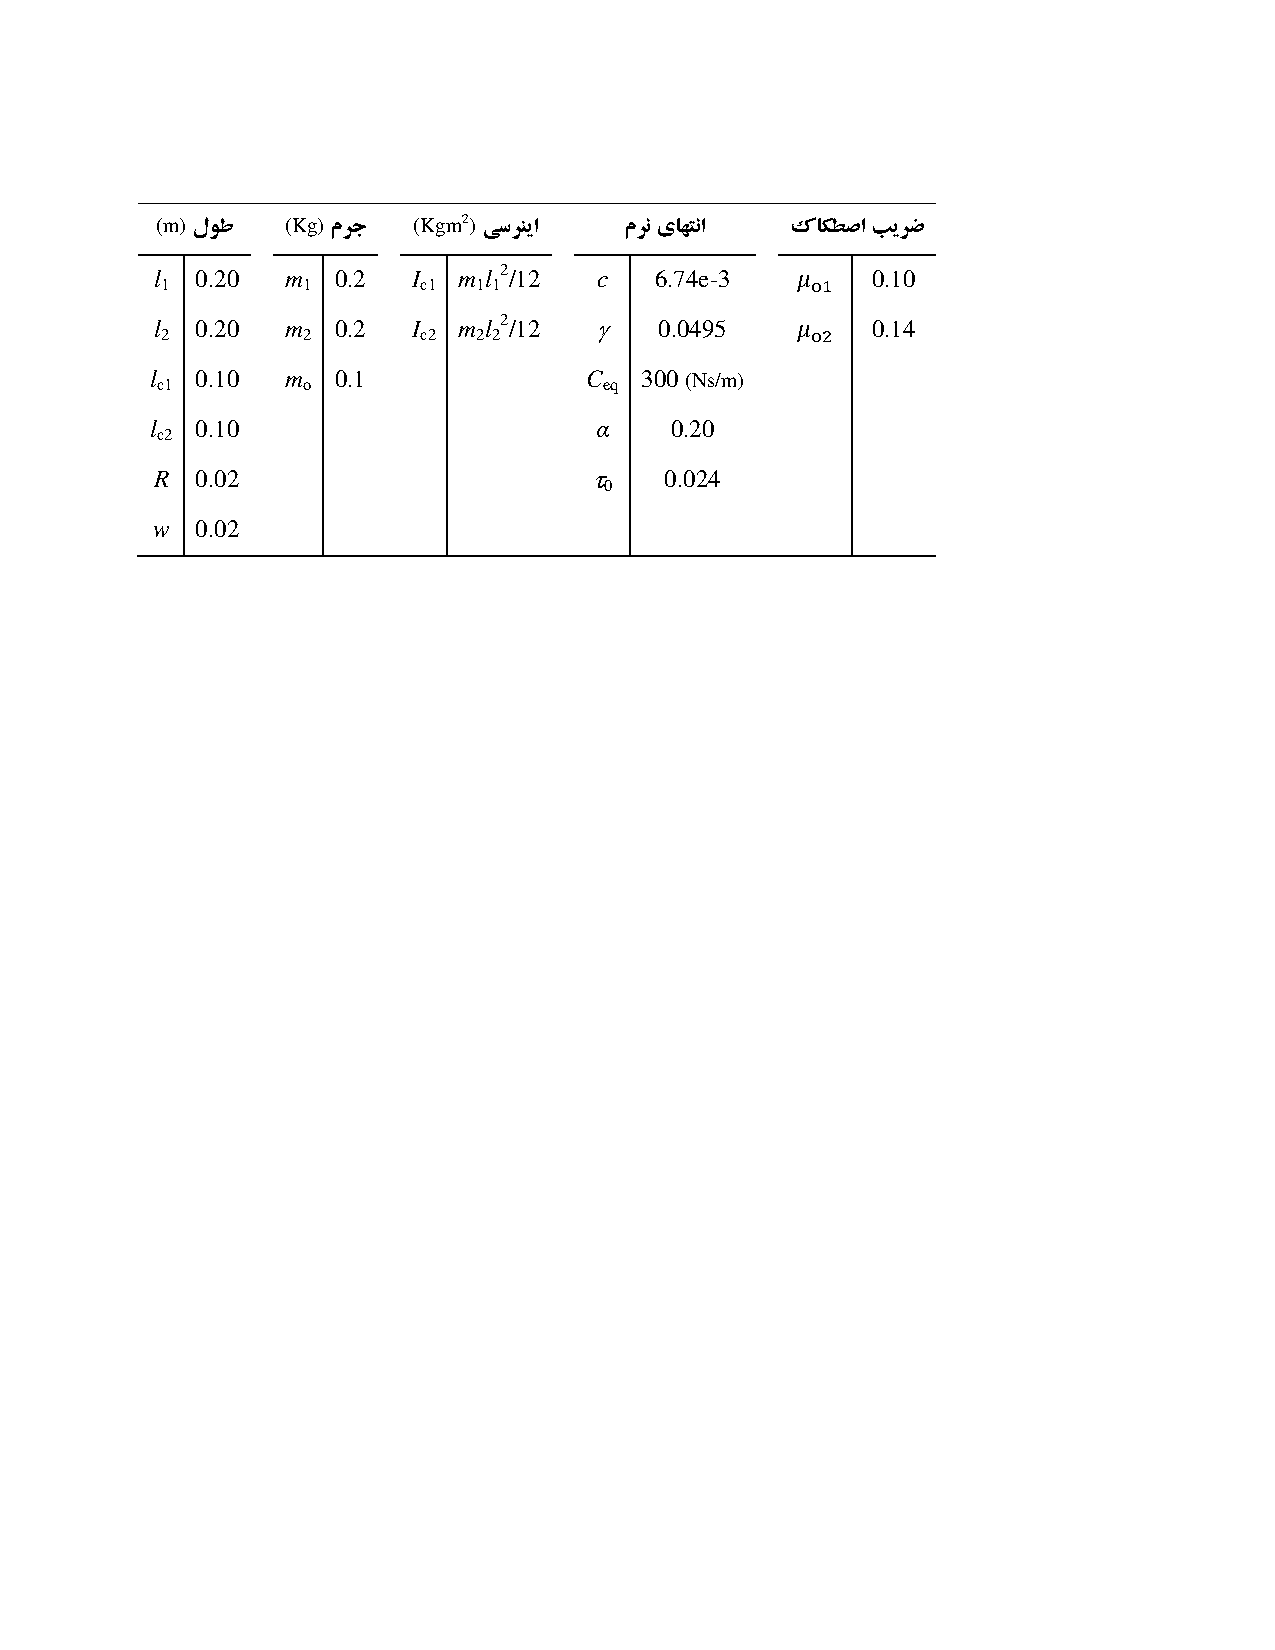
\includegraphics[scale=0.9]{Figures/SampleTable1.pdf} 
\end{tabular}
\vspace{-\baselineskip}
\label{Tbl:SampleTable1}
\end{table}

\begin{table}[!htb]
\caption{مقايسه‌ی روش‌هاي برداشت انرژي مبتني بر لرزش‌هاي مکانيکی}
\centering
\begin{tabular}{@{}|p{.15\textwidth}|p{.25\textwidth}|p{.25\textwidth}|p{.25\textwidth}|@{}}
\hline
روش
& 
چگالی انرژی
& 
ابعاد
& 
عیب اصلی
\\ \hline \hline
پیزوالکتریک
& 
$\mathrm{mJ/cm^3}$ 35/4
& 
بزرگ
& 
ولتاژ خروجی کم
\\ \hline
الکترومغناطیس
& 
$\mathrm{mJ/cm^3}$ 24/8
& 
بزرگ
& 
ولتاژ خروجی بسیار کم
\\ \hline
الکترواستاتیک
& 
$\mathrm{mJ/cm^3}$ 4
& 
فشرده در تراشه‌ها
& 
نیاز به منبع شارژ اولیه
\\ \hline
\end{tabular}
\label{Tbl:SampleTable2}
\vspace{-\baselineskip}
\end{table}

نمونه‌ای از یک رابطه به‌صورت
\begin{equation}
p\left( r \right) = {C_k}\frac{N}{{\pi {a^2}}}{\left[{1 - {{\left( {\frac{r}{a}} \right)}^k}} \right]^{\frac{1}{k}}},
\label{Eq:Pressure}
\end{equation}
است. در رابطه
\ref{Eq:Pressure}،
$N$
نیروی عمودی است. نمونه‌ای از استفاده از روابط متوالی به‌صورت
\begin{equation}
\sum \limits_{i = 1}^{k + 1} {E_s}\left( i \right) - T \sum \limits_{i = 1}^k {P_s}\left( i \right) \le B_s^{max},\quad k = 1, \ldots ,N - 1,
\label{Eq:batterysource}
\end{equation}\vspace{-\baselineskip}
\begin{equation}
\sum \limits_{i = 1}^{k + 1} {E_r}\left( i \right) - T \sum \limits_{i = 1}^k {P_r}\left( i \right) \le B_r^{max},\quad k = 1, \ldots ,N - 1,
\label{Eq:batteryrellay}
\end{equation}
است. نمونه‌ای از یک قضیه و تبصره نیز در ادامه آورده شده است.
\begin{theorem}
اگر ظرفیت باتری‌ها به اندازه کافی بزرگ باشد، جواب بهینه‌ی 
$P_s^*(i)$
و
$P_r^*(i)$
وجود دارد به نحوی که تابع هدف را بیشینه می‌کند و در رابطه‌ی زیر صدق می‌کند:
\begin{equation}
C\left( {{{\left| {{h_{sr}}\left( i \right)} \right|}^2}{P_s}^*\left( i \right)} \right) \ge C\left( {{{\left| {{h_{sd}}\left( i \right)} \right|}^2}{P_s}^*\left( i \right)} \right) + C\left( {{{\left| {{h_{rd}}\left( {i + 1} \right)} \right|}^2}P_r^*\left( {i} \right)} \right).
\label{Eq:theorem1}
\end{equation}

\begin{proof}
بار دیگر فرم تابع هدف را در نظر می‌گیریم. لازم به ذکر است اینجا تابع هدف یک تابع دومتغیره است.
\begin{equation}
{R({\mathbf{P}_s},{\mathbf{P}_r}) = {\frac{1}{2}\sum\limits_{i = 1}^N {\min } \left\{ {C\left( {{{\left| {{h_{sr}}\left( i \right)} \right|}^2}{P_s}\left( i \right)} \right),} C\left( {{{\left| {{h_{sd}}\left( i \right)} \right|}^2}{P_s}\left( i \right)} \right) \right\} }}.
\end{equation}
حال بلوک
$i$ام
را در نظر می‌گیریم. اگر رابطه‌ی
\ref{Eq:theorem1}
برای
$i$
برقرار نباشد، به عبارت دیگر اگر داشته باشیم،
\begin{equation}
C\left( {{{\left| {{h_{sr}}\left( i \right)} \right|}^2}{P_s}^*\left( i \right)} \right) < C\left( {{{\left| {{h_{sd}}\left( i \right)} \right|}^2}{P_s}^*\left( i \right)} \right) + C\left( {{{\left| {{h_{rd}}\left( {i + 1} \right)} \right|}^2}P_r^*\left( {i + 1} \right)} \right),
\label{Eq:theorem1(2)}
\end{equation}
بنابراین
\begin{equation}
C\left( {{{\left| {{h_{sr}}\left( i \right)} \right|}^2}{P_s}^*\left( i \right)} \right)+ C\left( {{{\left| {{h_{sd}}\left( i \right)} \right|}^2}{P_s}^*\left( i \right)} \right) =C\left( {{{\left| {{h_{sr}}\left( i \right)} \right|}^2}{P_s}^*\left( i \right)} \right).
\end{equation}
پس در تابع هدف مسئله، مقدار بهینه‌ی مسئله برابر عبارت سمت چپ رابطه‌ی
\ref{Eq:theorem1(2)}
شده است و آرگومان دوم و  هم‌چنین مقدار
$P_r^*(i)$
هیچ نقشی در مقدار بهینه ندارد. بنابراین می‌توانیم 
$P_r^*(i)$
را آنقدر کاهش دهیم تا در رابطه‌ی
\ref{Eq:theorem1(2)}
تساوی برقرار شود بدون آنکه مقدار بهینه‌ی مسئله تغییر کند.
\end{proof}
\label{theorem1}
\end{theorem}

\begin{remark}
از قضیه‌ی
\ref{theorem1}
نتیجه می‌گیریم که جواب بهینه‌ی مسئله‌ی
\lr{P}
در حالت کلی یکتا نیست. به طور مثال وقتی مقدار انرژی برداشت‌شده در رله خیلی بیشتر از این انرژی در منبع باشد مسئله می‌تواند جواب‌های زیادی داشته باشد. بنابراین همواره می‌توان برای صرفه‌جویی در مصرف انرژی، بدون کاهش مقدار نرخ گذردهی سیستم، کمترین مقدار توان را برای رله انتخاب کرد. بنابراین با توجه به رابطه
\begin{equation}
C\left( {{{\left| {{h_{sr}}\left( i \right)} \right|}^2}{P_s}^*\left( i \right)} \right) 
\ge C\left( {{{\left| {{h_{sd}}\left( i \right)} \right|}^2}{P_s}^*\left( i \right)} \right) + C\left( {{{\left| {{h_{rd}}\left( {i} \right)} \right|}^2}P_r^*\left( {i} \right)} \right),
\label{Eq:remark1}
\end{equation}
و با  استفاده از رابطه
\ref{Eq:remark1}
خواهیم داشت،
\begin{equation}
{R_r}(i) = \min \left\{ {C\left( {{{\left| {{h_{rd}}(i)} \right|}^2}{P_r}(i)} \right),C\left( {{{\left| {{h_{sr}}(i)} \right|}^2}{P_s}(i)} \right)} \right\}.
\end{equation}

بنابراین می‌توان با انتخاب کمترین توان و نرخ برای رله از مصرف بی‌رویه‌ی انرژی جلوگیری کرد. فرض بزرگ بودن ظرفیت باتری‌ به این دلیل است که اگر ظرفیت باتری محدود باشد برای کاهش
$P_r^*(i)$
با محدودیت مواجه هستیم. چون در صورت کاهش بی از حد توان رله ممکن است از ناحیه‌ی شدنی مسئله خارج شویم. به هر حال برای هر دو حالت ظرفیت نامحدود و محدود باتری جواب مسئله یکتا نیست و همواره می‌توان با کاهش توان رله مصرف انرژی را کاهش داد.
\end{remark}




